\chapter{DESAIN DAN IMPLEMENTASI}
\label{chap:desainimplementasi}

% Ubah bagian-bagian berikut dengan isi dari desain dan implementasi
\section{Deskripsi Sistem}
\label{sec:deskripsisistem}

Sistem terdiri dari tiga proses utama yaitu Pengambilan data, \textit{Training} data, Pembuatan \textit{Lookup Table}, dan yang terakhir adalah membaca data dari \textit{Lookup Table} tersebut sehingga menjadi data yang telah terkalibrasi.

\section{Pengambilan data
  \label{sec:pengambilandata}}

Hal yang dilakukan sebelum pengambilan data adalah menyiapkan robot dan marker yang telah dibuat sebelumnya. 

\begin{figure}[H]
  \centering
  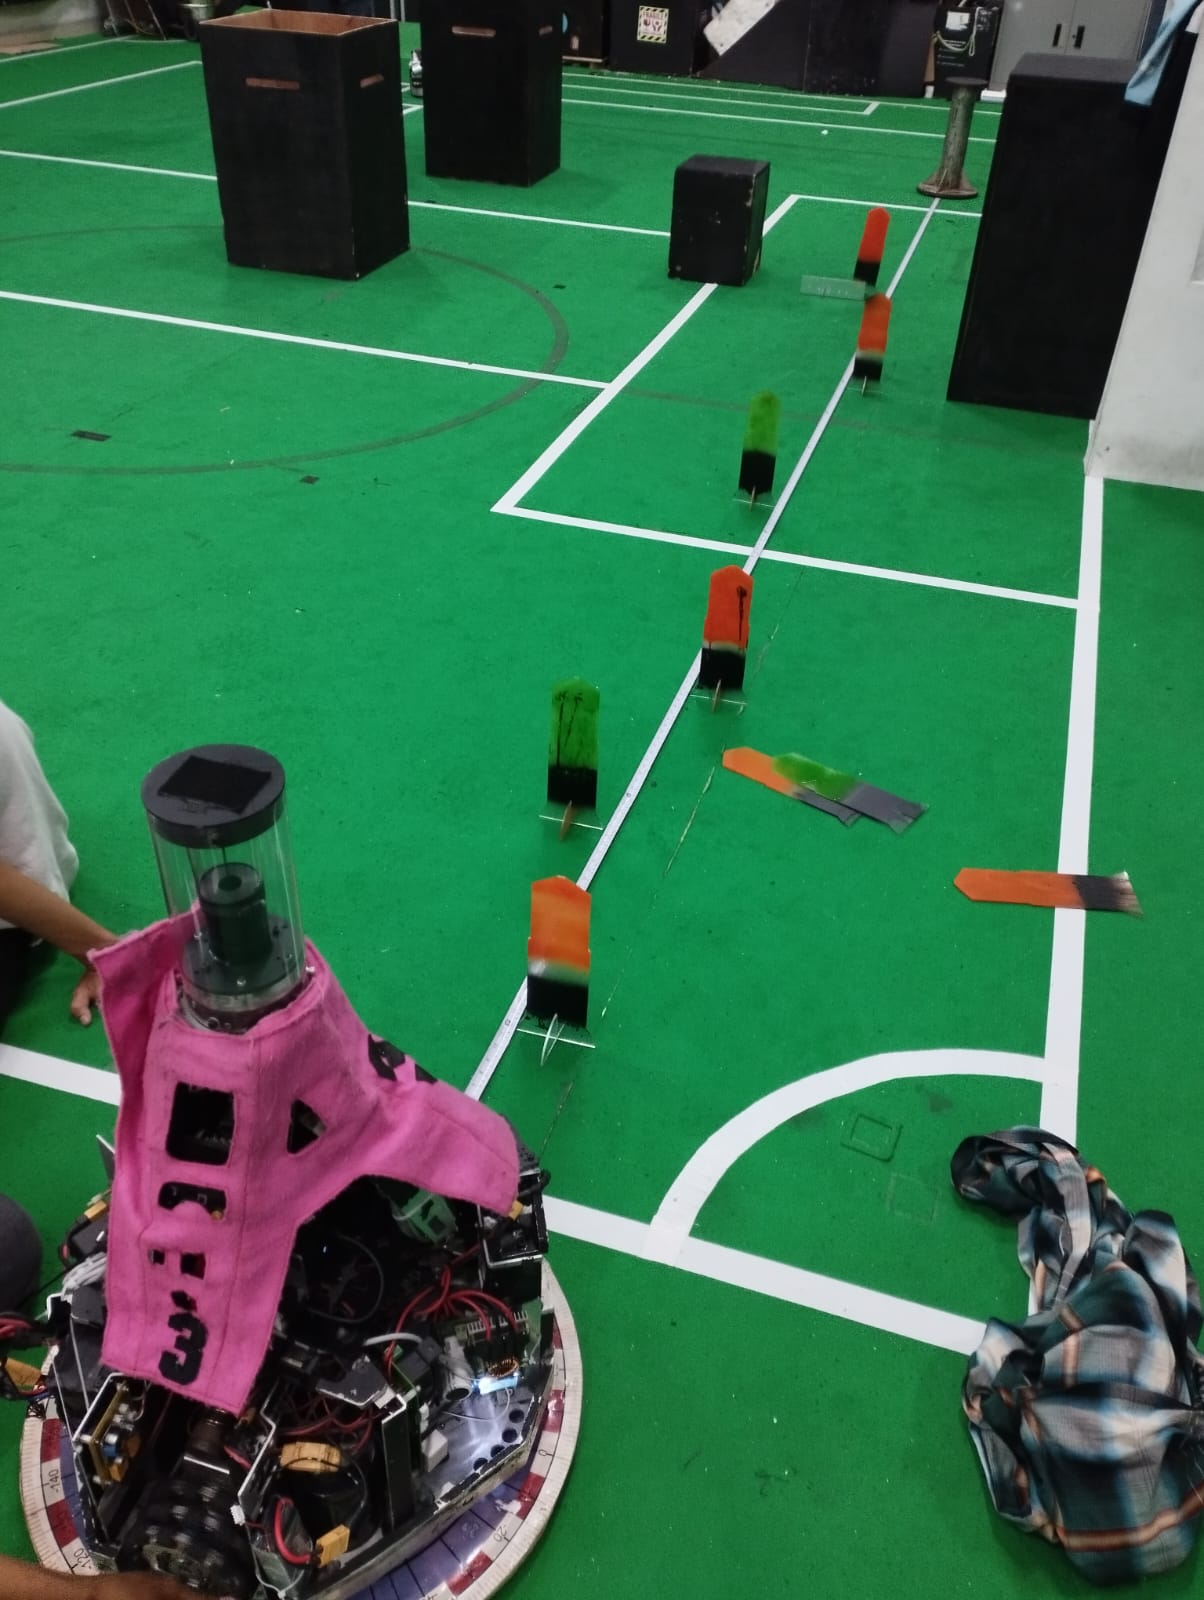
\includegraphics[scale=0.20]{gambar/ambil_data.jpeg}
  \caption{Persiapan robot.}
  \label{fig:persiapanrobot}
\end{figure}

Dikarenakan robot tidak memiliki display, maka untuk mengakses kamera perlu dilakukan dengan mengakses melalui program web yang telah disediakan oleh robot. Berikut adalah program robot untuk mengakses kamera dan mengirim ke web mengunakan \textit{websocket}.

\lstinputlisting[
  language=C++,
  caption={Program akses kamera.},
  label={lst:akseskamera}
]{program/akses_kamera.cpp}

\lstinputlisting[
  language=C++,
  caption={Program publish kamera.},
  label={lst:publishkamera}
]{program/publish_kamera.cpp}

\lstinputlisting[
  language=JavaScript,
  caption={Program akses kamera melalu web.},
  label={lst:kameraweb}
]{program/kamera_web.js}

Setelah software dan hardware telah disiapkan maka yang dilakukan selanjuatnya adalah mengambil data dari kamera. Data yang diambil adalah sebagai berikut:
\begin{figure}[H]
  \centering
  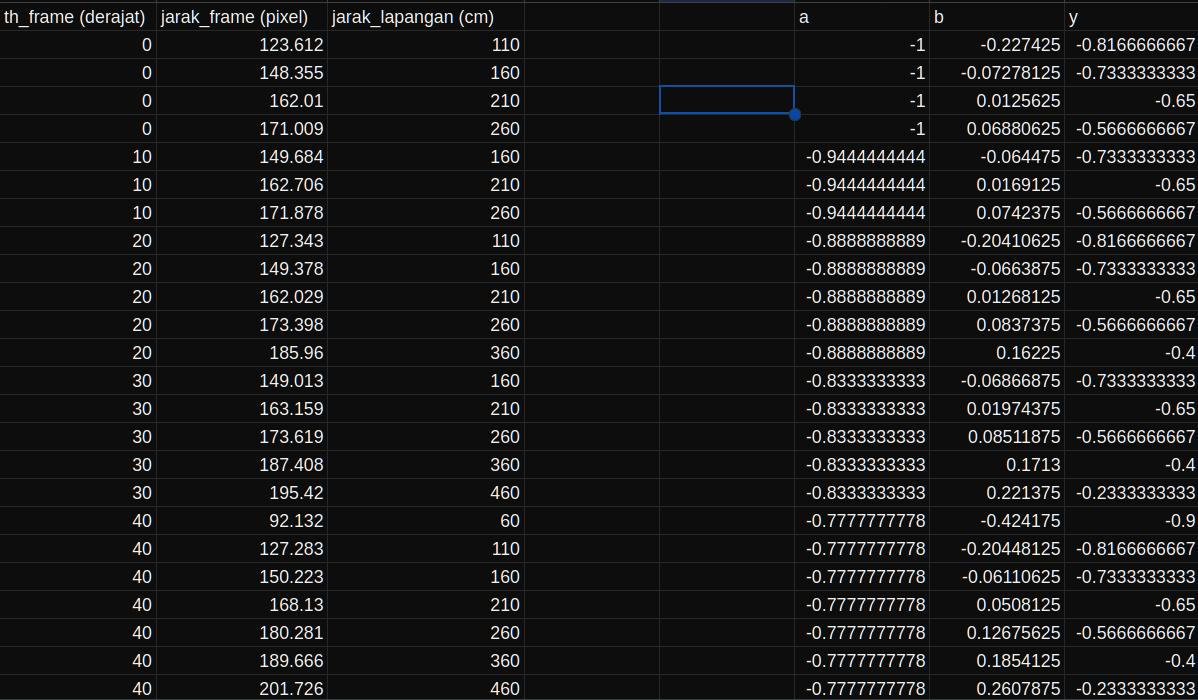
\includegraphics[scale=0.50]{gambar/data.jpg}
  \caption{Data \textit{training}.}
  \label{fig:datatraining}
\end{figure}

\section{\textit{Training} data
  \label{sec:trainingdata}}

Data yang telah diambil kemudian diolah dengan menggunakan program \textit{training} data. Program ini menggunakan metode \textit{Neural Network} untuk mengolah data tersebut. Berikut adalah program \textit{training} data.

% Contoh input potongan kode dari file
\lstinputlisting[
  language=Python,
  caption={Program \textit{train} data.},
  label={lst:traindata}
]{program/train.py}

\section{Pembuatan \textit{Lookup Table}
  \label{sec:pembuatanlut}}

Setelah data di-\textit{train} maka data tersebut akan dijadikan \textit{Lookup Table}. \textit{Lookup Table} ini berisi data-data yang telah di-\textit{train} sebelumnya. Berikut adalah program pembuatan \textit{Lookup Table}.

\lstinputlisting[
  language=Python,
  caption={Program pembuatan \textit{Lookup Table}.},
  label={lst:pembuatanlut}
]{program/save_lut.py}

\section{Pembacaan \textit{Lookup Table}
  \label{sec:pembacaanlut}}

Setelah \textit{Lookup Table} dibuat maka yang terakhir adalah membaca data dari \textit{Lookup Table} tersebut. Proses tersebut dilakukan pada robot. Berikut adalah program pembacaan \textit{Lookup Table}.

\lstinputlisting[
  language=C++,
  caption={Program membaca \textit{Lookup Table}.},
  label={lst:membacalut}
]{program/read_lut.cpp} 
